\documentclass[10pt,aspectratio=169]{beamer}

\usepackage[T1]{fontenc}
\usepackage{lmodern}

\usepackage{amsmath,amssymb,mathtools}
\usepackage{bm}
\usepackage{cancel}
\usepackage{empheq}
\usepackage{graphicx}
\usepackage{array,booktabs,tabularx,tabulary,multirow}
\usepackage{tikz}
\usepackage{hyperref}
\usepackage{feynmp}

\newcolumntype{V}{>{\centering\arraybackslash} m{.2\linewidth} }

\usetikzlibrary{arrows,matrix,shapes,positioning}
\usetikzlibrary{calc}
\usetikzlibrary{mindmap}
\usetikzlibrary{shadows.blur}

\newcommand*\widefbox[1]{\fbox{\hspace{0.5em}#1\hspace{0.5em}}}

\DeclareGraphicsRule{*}{mps}{*}{}
\graphicspath{{./figures/}}

\title{Dark Matter Predictions in $E_6$ Inspired SUSY Models}

\author{D.~Harries\\
  {\scriptsize
    (IPNP, Charles University in Prague)}\\
  \vspace{25pt}
  { \scriptsize
    Based on:\\[3mm]
  }
  { \tiny
    \href{https://doi.org/10.1016/j.physletb.2016.06.040}{%
      P.~Athron, D.~Harries, R.~Nevzorov, and A.~G.~Williams,
      Phys.~Lett.~\textbf{B760}, 19 (2016)}
         [\href{https://arxiv.org/abs/1512.07040}{arXiv:1512.07040}]\\[1mm]
    \href{https://doi.org/10.1007/JHEP12(2016)128}{%
      P.~Athron, D.~Harries, R.~Nevzorov, and A.~G.~Williams,
      JHEP \textbf{12}, 128 (2016)}
         [\href{https://arxiv.org/abs/1610.03374}{arXiv:1610.03374}]
  }
}

\titlegraphic{
  \begin{center}
    \hspace*{\fill}
    
\includegraphics[scale=0.3]{uk_logo}
    \hspace*{\fill}
  \end{center}
}

\date[\'{U}TF, Charles University in Prague]{April 9, 2018}

\usetheme{CambridgeUS}

\setbeamertemplate{headline}[default]{}
\setbeamertemplate{footline}[page number]{}
\setbeamertemplate{navigation symbols}{}

\begin{document}

\begin{frame}[plain]
  \titlepage
\end{frame}

\section{Motivation}

\begin{frame}
  \frametitle{Evidence for DM}
  \begin{columns}[t]
    \begin{column}{0.3\textwidth}
      \vspace*{-20pt}
      \begin{figure}
        \centering
        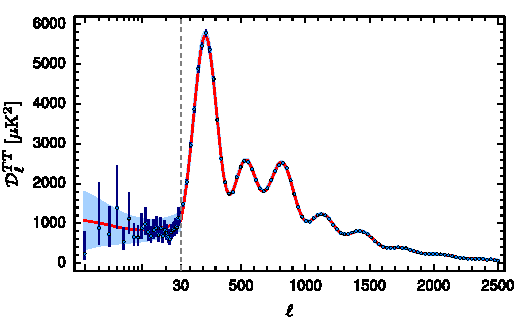
\includegraphics[width=0.95\textwidth]{cmb_power_spectrum}
      \end{figure}
      \vspace*{-25pt}
      \begin{center}
        { \tiny [\href{http://arxiv.org/abs/1502.02114}{%
              arXiv:1502.02114}] }
      \end{center}
      \vspace*{-20pt}
      \begin{center}
        CMB measurements
      \end{center}
      \vspace*{-15pt}
      \begin{figure}
        \centering
        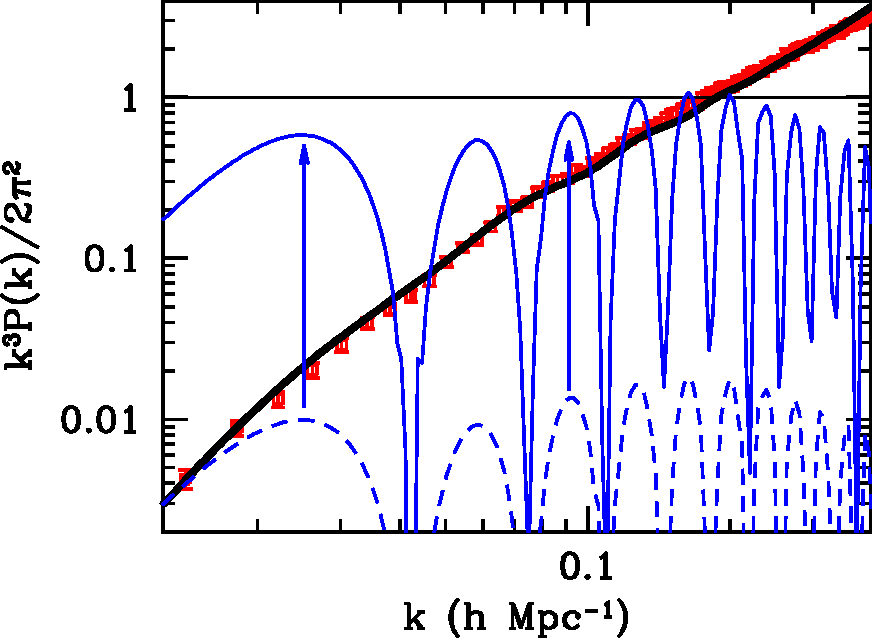
\includegraphics[width=0.95\textwidth]{matter_power_spectrum}
      \end{figure}
      \vspace*{-20pt}
      \begin{center}
        { \tiny [\href{http://arxiv.org/abs/1112.1320}{%
              arXiv:1112.1320}] }
      \end{center}
      \vspace*{-20pt}
      \begin{center}
        Structure formation
      \end{center}
    \end{column}
    \begin{column}{0.3\textwidth}
      \begin{figure}
        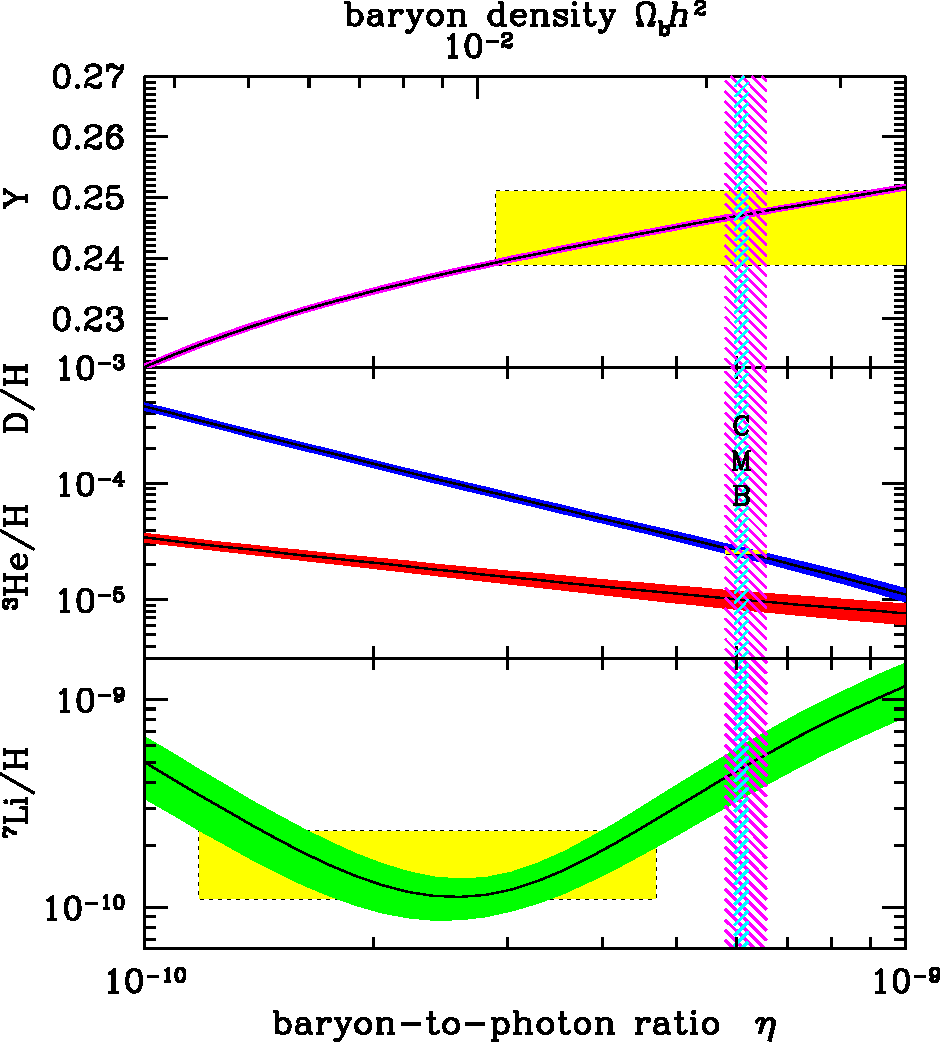
\includegraphics[width=\textwidth]{bbn}
      \end{figure}
      \vspace*{-25pt}
      \begin{center}
        { \tiny [\href{http://pdg.lbl.gov/2017/reviews/rpp2017-rev-bbang-nucleosynthesis.pdf}{%
              PDG 2017}] }
      \end{center}
      \vspace*{-15pt}
      \begin{center}
        BBN
      \end{center}
    \end{column}
    \begin{column}{0.3\textwidth}
      \vspace*{-20pt}
      \begin{figure}
        \centering
        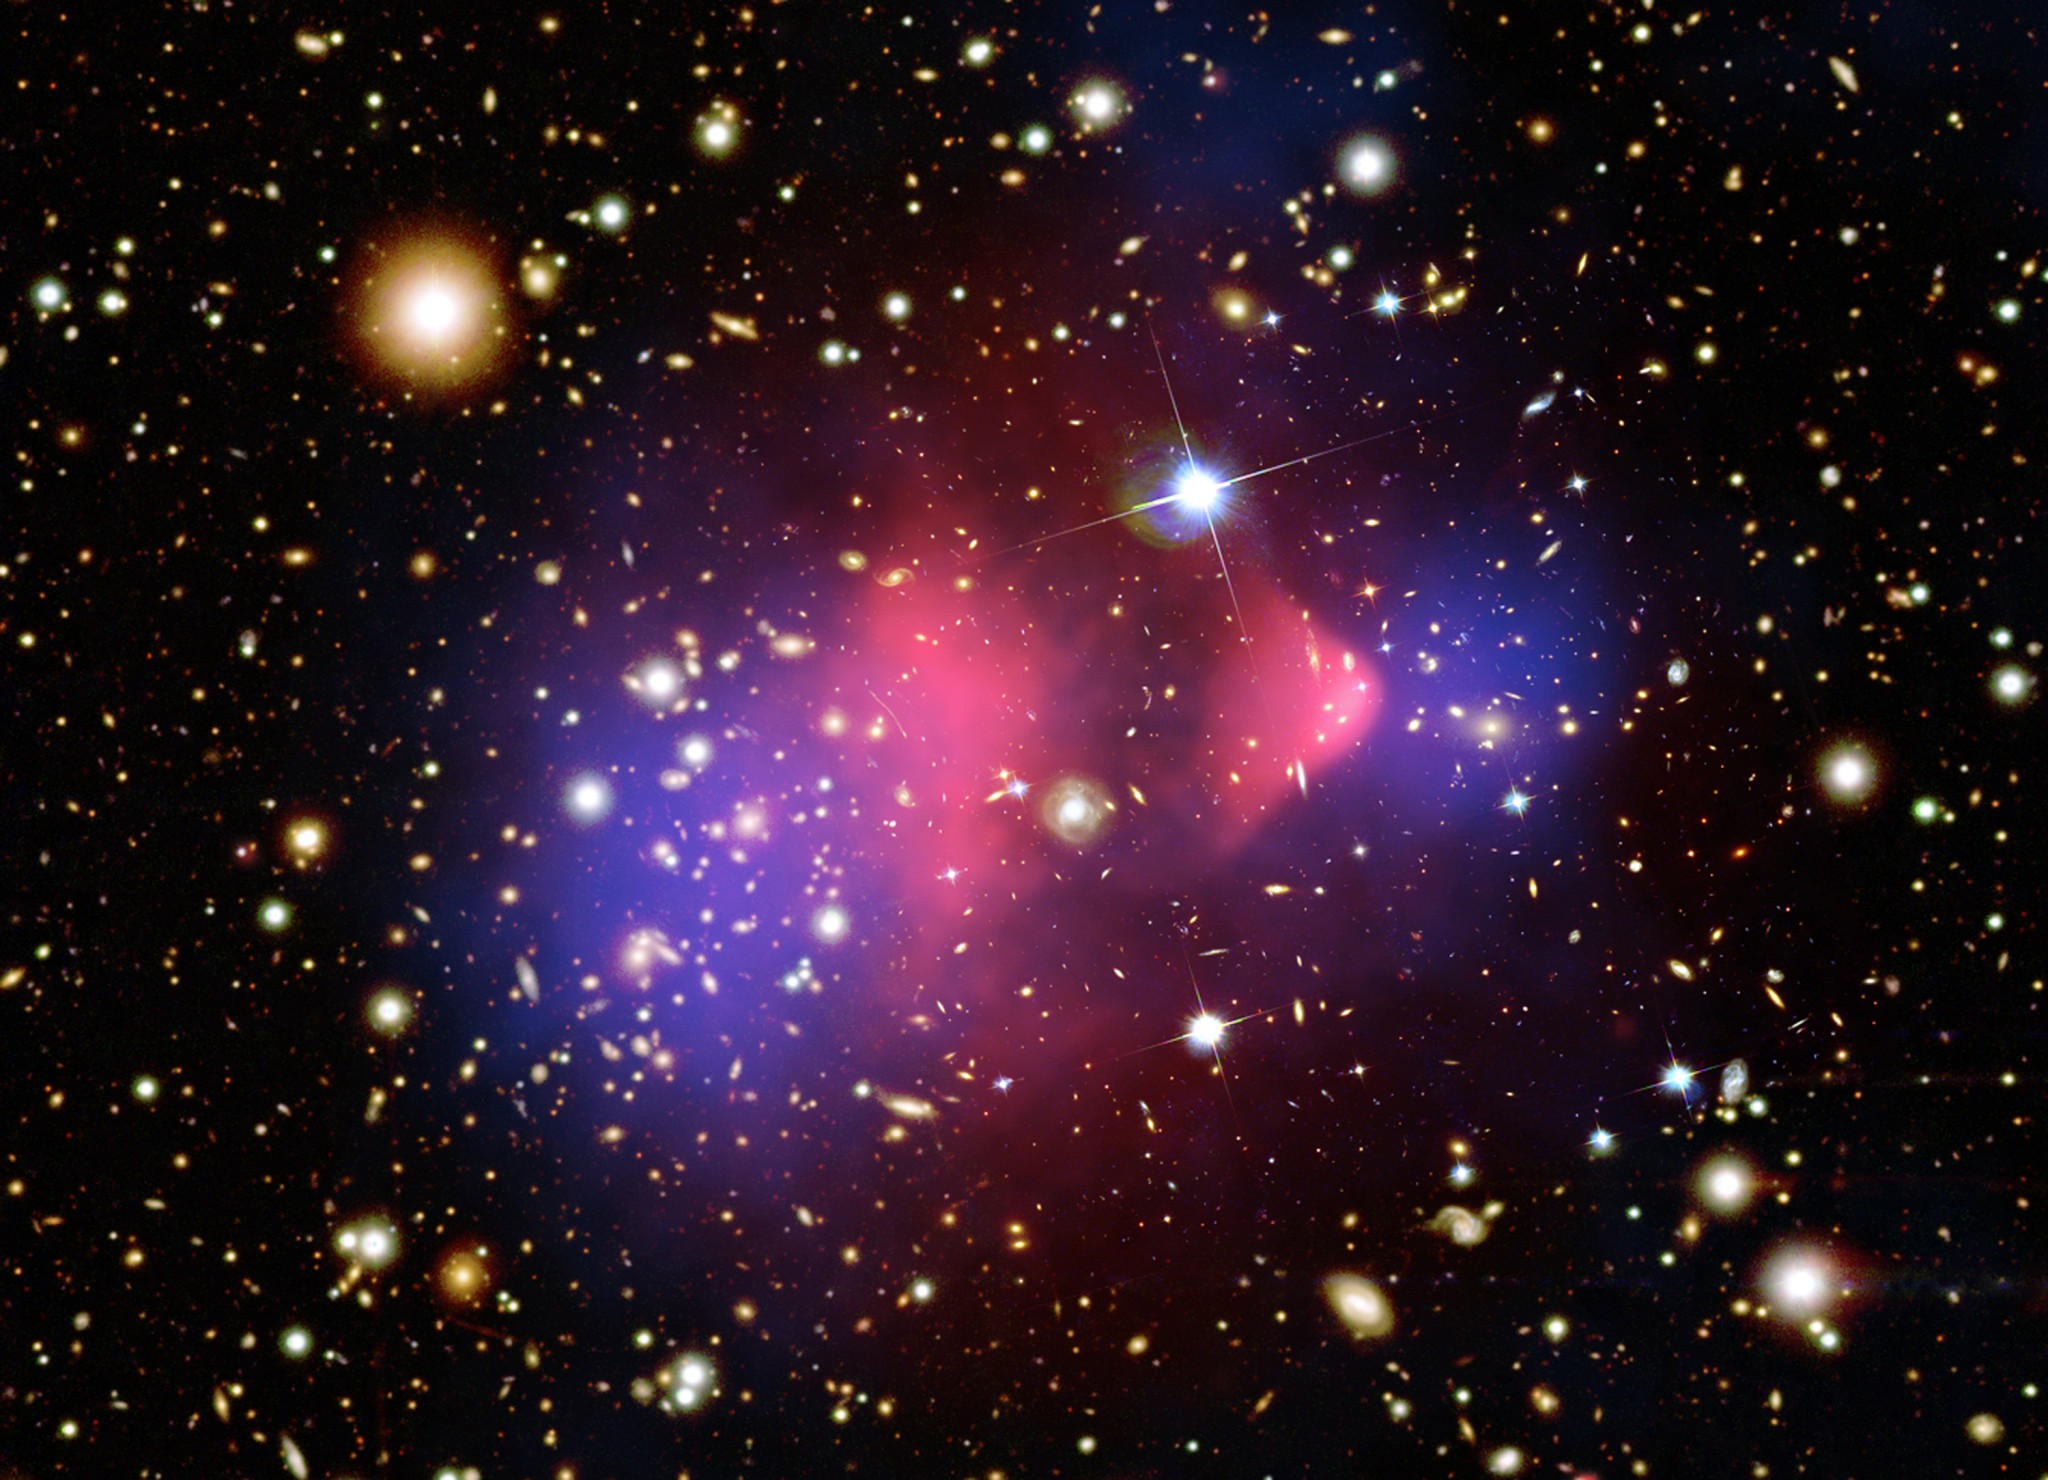
\includegraphics[width=0.85\textwidth]{bulletcluster}
      \end{figure}
      \vspace*{-25pt}
      \begin{center}
        {\tiny [\href{https://apod.nasa.gov/apod/ap060824.html}{APOD/NASA}]}
      \end{center}
      \vspace*{-20pt}
      \begin{center}
        Galaxy cluster mergers
      \end{center}
      \vspace*{-10pt}
      \begin{figure}
        \centering
        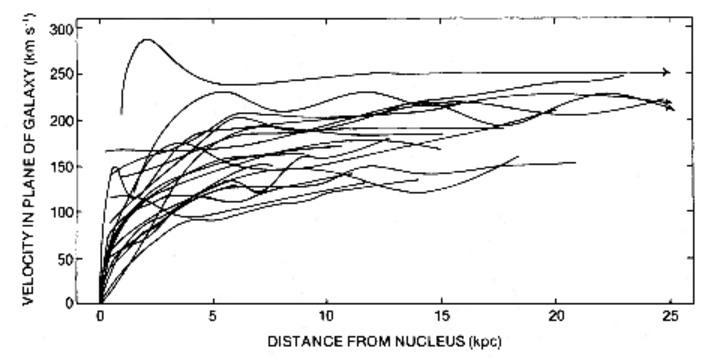
\includegraphics[width=\textwidth]{rotation_curves}
      \end{figure}
      \vspace*{-25pt}
      \begin{center}
        { \tiny [V.~C.~Rubin, N.~Thonnard, and W.~K.~Ford, Jr.,
            \href{http://doi.org/10.1086/158003}{%
              Astrophys.~J.~\textbf{238} (1980) 471}] }
      \end{center}
      \vspace*{-17pt}
      \begin{center}
        Galaxy rotation curves
      \end{center}
    \end{column}
  \end{columns}
\end{frame}

\begin{frame}
  \frametitle{DM Candidates}
  \begin{figure}
    \centering
    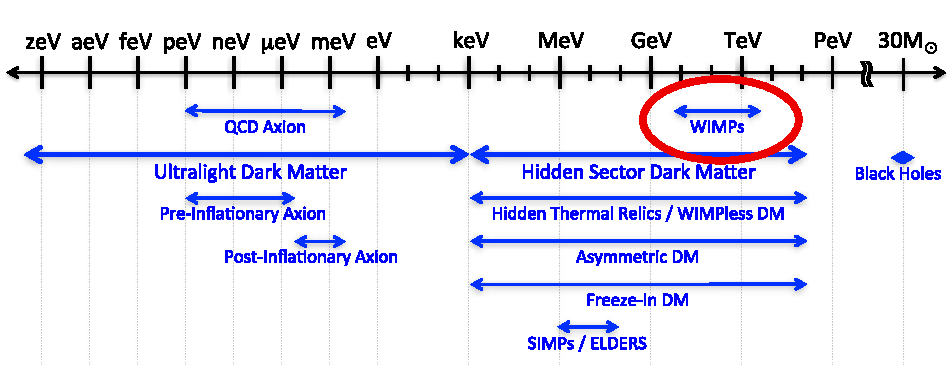
\includegraphics[width=\textwidth]{dmcandidates}
  \end{figure}
  \vspace*{-20pt}
  \begin{center}
    {\tiny [\href{http://arxiv.org/abs/1707.04591}{%
          arXiv:1707.04591}]}
  \end{center}
\end{frame}

\begin{frame}
  \frametitle{WIMP DM: Relic Density}
  \begin{columns}[t]
    \begin{column}{0.5\textwidth}
      \begin{itemize} \itemsep1em
      \item Relic density of standard WIMPs results from
        freeze-out ($Y = n_\chi / s$),
        \begin{equation*}
          \frac{d Y}{d t} = - s \langle \sigma v \rangle ( Y^2
          - Y^2_{\text{eq.}} )
          \Rightarrow
          \Omega_\chi h^2 = \frac{m_\chi s_0 h^2}{\rho_c} Y_\infty
        \end{equation*}
      \item ``WIMP miracle'': for $m_\chi \sim$ GeV $-$ TeV,
        $g_\chi \sim g_{\text{weak}}$,
        \begin{equation*}
          \Omega_\chi \sim \frac{m_\chi^2}{g_\chi^4} \sim \Omega_{\text{DM}}
        \end{equation*}
      \item \alert{$\Omega_\chi h^2 > (\Omega_{\text{DM}} h^2)_{\text{Planck}}$
        $\Rightarrow$ model ruled out}
        \begin{itemize} \itemsep0.5em
        \item N.B. $\Omega_\chi h^2 < (\Omega_{\text{DM}} h^2)_{\text{Planck}}$
          allowed
        \item e.g., multiple DM candidates $\chi_i$, $\sum_i \Omega_{\chi_i} =
          \Omega_{\text{DM}}$
        \end{itemize}
      \end{itemize}
    \end{column}
    \begin{column}{0.5\textwidth}
      \vspace*{-20pt}
      \begin{figure}
        \centering
        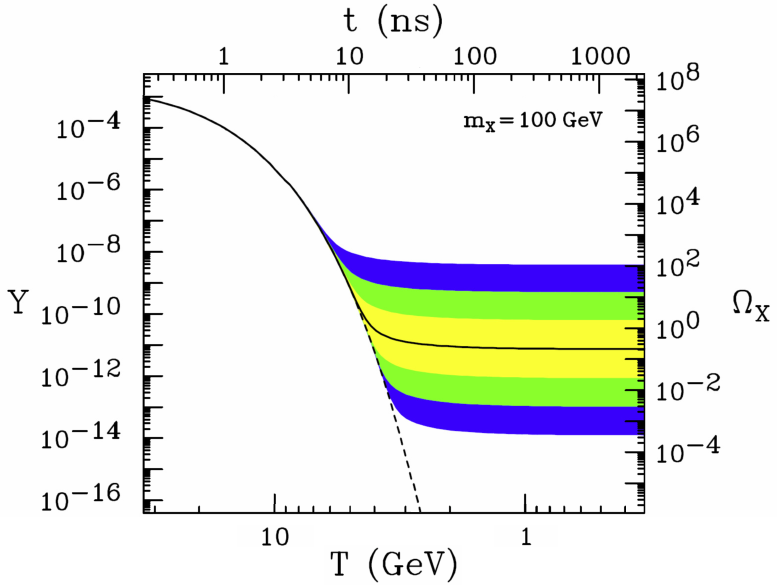
\includegraphics[width=\textwidth]{freezeout}
      \end{figure}
      \vspace*{-20pt}
      \begin{center}
        { \tiny [\href{http://arxiv.org/abs/1003.0904}{%
              arXiv:1003.0904}] }
      \end{center}
      \begin{center}
        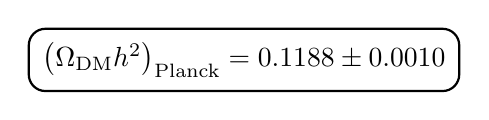
\begin{tikzpicture}
          \node[rectangle, draw, fill = white, rounded corners = 6pt,
          thick, inner sep = 0.5em]{%
            $\left ( \Omega_{\text{DM}} h^2 \right )_{\text{Planck}}
            = 0.1188 \pm 0.0010$
          };
        \end{tikzpicture}
      \end{center}
    \end{column}
  \end{columns}
\end{frame}

\begin{frame}
  \frametitle{Constraining WIMP Models}
  \begin{columns}[t]
    \begin{column}{0.5\textwidth}
      \begin{figure}
        \centering
        \includegraphics[height=0.4\textwidth]{dmsignals}
      \end{figure}
      \vspace*{-10pt}
      \begin{itemize} \itemsep1em
      \item Multiple approaches: {\color{blue} direct detection}
        ($\rightarrow$), indirect detection ($\uparrow$), collider searches
        ($\downarrow$)
      \item Direct detection: observe nuclear recoil in DM-nucleus interaction,
        \begin{equation*}
          \frac{d R}{d E} =\frac{1}{2 m_\chi m_r^2} {\color{red}
            \sigma(q) \rho_{\chi, \text{local}}} \eta(v_{\text{min}}(E), t)
        \end{equation*}
      \end{itemize}
    \end{column}
    \begin{column}{0.5\textwidth}
      \begin{itemize}\itemsep1em
      \item \alert{LUX, XENON1T, $\ldots$ $\Rightarrow$ stringent limits on
        $\sigma^{(SI/SD)}$:}
      \end{itemize}
      \begin{figure}
        \centering
        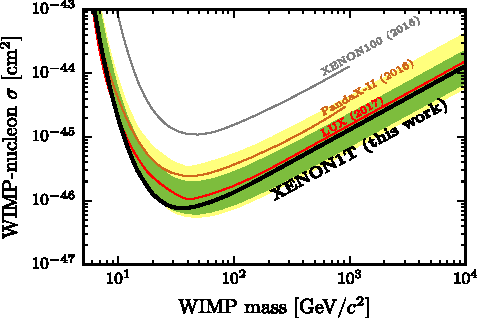
\includegraphics[width=\textwidth]{xenon1t_si_limit}
      \end{figure}
      \vspace*{-20pt}
      \begin{center}
        {\tiny [\href{http://arxiv.org/abs/1705.06655}{%
              arXiv:1705.06655}]}
      \end{center}
    \end{column}
  \end{columns}
\end{frame}

\begin{frame}
  \frametitle{The MSSM}
  \begin{columns}
        \begin{column}{0.5\textwidth}
      \begin{figure}
        \centering
        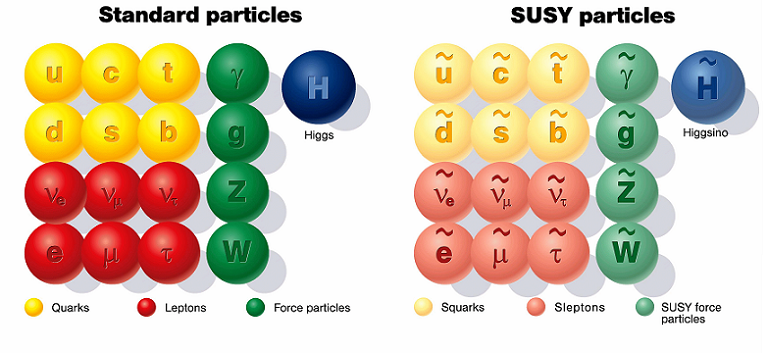
\includegraphics[width=\textwidth]{susyparticles_sm}
      \end{figure}
      \vspace*{-20pt}
      \begin{center}
        {\tiny [\href{http://www.physics.gla.ac.uk/ppt/bsm.htm}{%
      http://www.physics.gla.ac.uk/ppt/bsm.htm}] }
      \end{center}
    \end{column}
    \begin{column}{0.5\textwidth}
      \begin{table}[h]
        \centering
        \scriptsize
        \begin{tabular}{cccccc}
          \toprule
          $\hat{\Phi}$ & $s = 0$ & $s = \frac{1}{2}$ & $SU(3)_C$ & $SU(2)_L$
          & $\sqrt{\frac{5}{3}} Q_i^Y$ \\
          \midrule
          $\hat{Q}_i$ & $\begin{pmatrix} \tilde{u}_{L} \\
            \tilde{d}_{L} \end{pmatrix}_i$
            & $\begin{pmatrix} u_{L} \\ d_L\end{pmatrix}_i$
            & $\mathbf{3}$ & $\mathbf{2}$ & $\frac{1}{6}$ \\[1em]
          $\hat{u}^c_i$ & $\tilde{u}^*_{iR}$ & $u^c_{iR}$
            & $\bar{\mathbf{3}}$ & $\mathbf{1}$ & $-\frac{2}{3}$ \\[0.5em]
          $\hat{d}^c_i$ & $\tilde{d}^*_{iR}$ & $d^c_{iR}$
            & $\bar{\mathbf{3}}$ & $\mathbf{1}$ & $\frac{1}{3}$ \\[0.5em]
          $\hat{L}_i$ & $\begin{pmatrix} \tilde{\nu}_{L} \\
              \tilde{e}_{L} \end{pmatrix}_i$
            & $\begin{pmatrix} \nu_{L}\\ e_L \end{pmatrix}_i$
            & $\mathbf{1}$ & $\mathbf{2}$ & $-\frac{1}{2}$ \\[1em]
          $\hat{e}^c_i$ & $\tilde{e}^*_{iR}$ & $e^c_{iR}$
            & $\mathbf{1}$ & $\mathbf{1}$ & $1$ \\[0.5em]
          $\hat{H}_d$ & $\begin{pmatrix} H_d^0 \\ H_d^- \end{pmatrix}$
            & $\begin{pmatrix} \tilde{H}_d^0 \\ \tilde{H}_d^- \end{pmatrix}$
            & $\mathbf{1}$ & $\mathbf{2}$ & $-\frac{1}{2}$ \\[1em]
          $\hat{H}_u$ & $\begin{pmatrix} H_u^+ \\ H_u^0 \end{pmatrix}$
            & $\begin{pmatrix} \tilde{H}_u^+ \\ \tilde{H}_u^0 \end{pmatrix}$
            & $\mathbf{1}$ & $\mathbf{2}$ & $\frac{1}{2}$ \\[1em]
            \bottomrule
        \end{tabular}
      \end{table}
    \end{column}
  \end{columns}
      \begin{empheq}[box=\widefbox]{align*}
        W_{\text{MSSM}} &= \mu ( \hat{H}_d \cdot \hat{H}_u )
        + y_{ij}^e \hat{e}^c_i ( \hat{L}_j \cdot \hat{H}_d )
        + y_{ij}^d \hat{d}^c_i ( \hat{Q}_j \cdot \hat{H}_d )
        + y_{ij}^u \hat{u}_i^c ( \hat{H}_u \cdot \hat{Q}_j ) \\
        & \quad {} {\color{red} - \epsilon_i \hat{L}_i \cdot \hat{H}_u
          + \frac{1}{2} \rho_{ijk} \hat{L}_i \cdot \hat{L}_j \hat{e}_k^c
          + \rho^\prime_{ijk} \hat{L}_i \cdot \hat{Q}_j \hat{d}_k^c
          + \frac{1}{2} \rho^{\prime\prime}_{ijk} \hat{u}_i^c
          \hat{d}_j^c \hat{d}_k^c }
      \end{empheq}
\end{frame}

\begin{frame}
  \frametitle{Neutralino DM}
  \begin{columns}[t]
    \begin{column}{0.5\textwidth}
      \begin{itemize} \itemsep1em
      \item Forbid $B$, $L$ violating interactions $\Rightarrow$
        impose {\color{blue} $R$-parity $\Leftrightarrow$
        matter parity}
        \begin{equation*}
          Z_2^R = (-1)^{3(B - L) + 2 s} , \quad
          Z_2^M = (-1)^{3 (B - L)}
        \end{equation*}
      \item $\Rightarrow$ lightest $R$-parity odd state (LSP) is
        {\color{blue} natural WIMP DM candidate} (provided $Q_{LSP} = 0$)
      \item Standard MSSM candidate is
        \begin{equation*}
          \tilde{\chi}_1^0 = N_{11} \tilde{H}_d^0 + N_{12} \tilde{H}_u^0
          + N_{13} \tilde{W}_3 + N_{14} \tilde{B}
        \end{equation*}
      \item Properties dependent on $m_{\tilde{\chi}_1^0}$, $N_{ij}$
        (i.e., $\mu$, soft breaking $M_1$, $M_2$)
      \end{itemize}
    \end{column}
    \begin{column}{0.5\textwidth}
      \begin{figure}
        \centering
        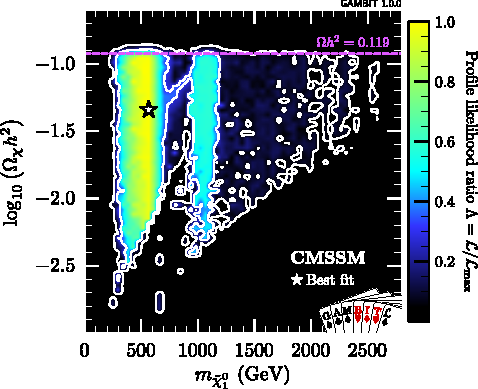
\includegraphics[width=0.9\textwidth]{gambit_gut_direct_detection}
      \end{figure}
      \vspace*{-20pt}
      \begin{center}
        { \tiny [\href{http://arxiv.org/abs/1705.07935}{%
              arXiv:1705.07935}] }
      \end{center}
    \end{column}
  \end{columns}
\end{frame}

\section{E$_6$ Inspired Models}

\begin{frame}
  \frametitle{E$_6$ Inspired Models}
  \begin{itemize} \itemsep1em
    \item Motivated by MSSM shortcomings, e.g., tree-level $m_{h_1}^2
      \leq M_Z^2 \cos^2 2\beta$ (\alert{``little hierarchy problem''}),
      \alert{$\mu$-problem}, $\nu$ masses, $\ldots$
    \item Lead to $U(1)$ extended models at low-energies:
      \begin{align*}
        E_6&\longrightarrow SO(10)\times U(1)_\psi \\
        &\longrightarrow SU(5)\times U(1)_\psi\times U(1)_\chi\\
        &\longrightarrow SU(3)_C\times SU(2)_L\times U(1)_Y\times
        U(1)_\psi\times U(1)_\chi\\
        &\longrightarrow SU(3)_C\times SU(2)_L\times U(1)_Y\times
        U(1)^\prime
      \end{align*}
    \item Resulting charges $Q' = Q_\chi \cos \theta_{E_6}
      + Q_\psi \sin \theta_{E_6}$
    \item Matter content fills complete $\mathbf{27}$ representations
      (anomaly cancellation)
      \begin{itemize}
      \item $\Rightarrow$ additional exotic states
      \end{itemize}
    \item Extra $D$- and $F$-terms $\Rightarrow$ {\color{blue}
      larger $m_{h_1}$}
    \item Break $U(1)^\prime$ with singlet $\Rightarrow$ {\color{blue}
      dynamically generate $\mu$ term}, massive $Z^\prime$
  \end{itemize}
\end{frame}

\begin{frame}
  \frametitle{The E$_6$SSM}
    \begin{columns}[t]
      \begin{column}{0.5\textwidth}
        \begin{itemize}
          \vfill
        \item $\tan\theta_{E_6} = \sqrt{15}$ $\Rightarrow$ $U(1)_N$
          under which right-handed neutrinos are uncharged
          \begin{itemize}
          \item allows $\nu$ masses via see-saw and
            successful baryogenesis [1]
          \end{itemize}
          \vfill
        \item Extra $\hat{L}_4$, $\hat{\overline{L}}_4$ from incomplete
          $\mathbf{27}^\prime$, $\mathbf{\overline{27}}^\prime$ for gauge
          unification
          \vfill
        \item Low-energy matter content from $\mathbf{27}$-plet:
          \begin{align*}
            &(\hat{Q}_i, \, \hat{u}^c_i, \, \hat{d}^c_i, \, \hat{L}_i, \,
            \hat{e}^c_i) + (\hat{D}_i, \, \hat{\overline{D}}_i)\\
            &\quad {} + (\hat{S}_{i}) + (\hat{H}^u_i) + (\hat{H}^d_i)
          \end{align*}
          \vfill
        \item Higgs doublets $\hat{H}^d_3$, $\hat{H}^u_3$ and one singlet
          $\hat{S}_3$ get VEVs ($\Rightarrow$ EWSB and break $U(1)_N$)
          \vfill
        \end{itemize}
      \end{column}
      \begin{column}{0.5\textwidth}
        \vspace{-40pt}
        \begin{table}[h]
          \centering
          \begin{tabular}{ccccc}
            \toprule
            & $SU(3)_C$ & $SU(2)_L$ & $\sqrt{\frac{5}{3}} Q_i^Y$
            & $\sqrt{40} Q_i^N$ \\
            \midrule
            $\hat{Q}_i$ & $\mathbf{3}$ & $\mathbf{2}$ & $\frac{1}{6}$ & $1$ \\
            $\hat{u}_i^c$ & $\mathbf{\overline{3}}$ & $\mathbf{1}$
            & $-\frac{2}{3}$ & $1$ \\
            $\hat{d}_i^c$ & $\mathbf{\overline{3}}$ & $\mathbf{1}$
            & $\frac{1}{3}$ & $2$ \\
            $\hat{L}_i$ & $\mathbf{1}$ & $\mathbf{2}$ & $-\frac{1}{2}$ & $2$ \\
            $\hat{e}_i^c$ & $\mathbf{1}$ & $\mathbf{1}$ & $1$ & $1$ \\
            $\hat{S}_i$ & $\mathbf{1}$ & $\mathbf{1}$ & $0$ & $5$ \\
            $\hat{H}_i^u$ & $\mathbf{1}$ & $\mathbf{2}$ & $\frac{1}{2}$
            & $-2$ \\
            $\hat{H}_i^d$ & $\mathbf{1}$ & $\mathbf{2}$ & $-\frac{1}{2}$
            & $-3$ \\
            $\hat{D}$ & $\mathbf{3}$ & $\mathbf{1}$ & $-\frac{1}{3}$ & $-2$ \\
            $\hat{\overline{D}}$ & $\mathbf{\overline{3}}$ &  $\mathbf{1}$
            & $\frac{1}{3}$ & $-3$ \\
            $\hat{L}_4$ & $\mathbf{1}$ & $\mathbf{2}$ & $-\frac{1}{2}$ & $2$ \\
            $\hat{\overline{L}}_4$ & $\mathbf{1}$ & $\mathbf{\overline{2}}$
            & $\frac{1}{2}$ & $-2$ \\
            \bottomrule
          \end{tabular}
        \end{table}
      \end{column}
    \end{columns}
    \vspace{-4pt}
    \begin{align*}
      \Aboxed{W_{\text{E}_6\text{SSM}} \approx y_{\tau} \hat{L}_3 \cdot
        \hat{H}^d_3 \hat{e}^c_3 + y_b \hat{Q}_3 \cdot \hat{H}^d_3 \hat{d}_3^c
        + y_t \hat{H}^u_3 \cdot \hat{Q}_3 \hat{u}_3^c + \lambda_i \hat{S}_3
        \hat{H}_i^d \cdot \hat{H}_i^u  + \kappa_i \hat{S}_3 \hat{D}_i
        \hat{\overline{D}}_i + \mu_L \hat{L}_4 \cdot \hat{\overline{L}}_4}
    \end{align*}
        {\tiny [1] S.~F.~King, S.~Moretti, and R.~Nevzorov,
          \href{http://doi.org/10.1103/PhysRevD.73.035009}{Phys.~Rev.~D
            \textbf{73}, 035009 (2006)}
          (\href{http://arxiv.org/abs/hep-ph/0510419}{hep-ph/0510419})}
\end{frame}

\begin{frame}
  \frametitle{Discrete Symmetries and DM in the E$_6$SSM}
  \begin{itemize}\itemsep0.8em
  \item Neutralino sector extended by ``inert'' $\tilde{S}_\alpha$,
    $\tilde{H}^{d,u}_{\alpha}$ $\Rightarrow$ DM candidate not MSSM-like in
    general
  \item General superpotential
    \begin{equation*}
      W \supset {\color{red} g_{ijk}^D} \hat{D}_i \hat{Q}_j \cdot \hat{Q}_k
      + {\color{red} \tilde{g}_{ijk}^E} \hat{e}_i^c \hat{D}_j \hat{u}_k^c
      + {\color{orange} y_{ijk}^U} \hat{u}_i^c \hat{H}_{uj} \cdot \hat{Q}_k
      + {\color{orange} y_{ijk}^D} \hat{d}_i^c \hat{Q}_j \cdot
      \hat{H}_{dk} + \ldots
    \end{equation*}
    $\Rightarrow$ impose {\color{red} exact $Z_2^{B/L}$} and {\color{orange}
      approximate $Z_2^H$} (compare single $R$-parity in MSSM)
    \item Resulting Higgs, singlet couplings
      \begin{equation*}
        W \supset \lambda \hat{S} \hat{H}_{d3} \cdot \hat{H}_{u3}
        + \lambda_{\alpha\beta} \hat{S} \hat{H}_{d\alpha} \cdot
        \hat{H}_{u\beta} + \tilde{f}_{\alpha\beta} \hat{S}_\alpha
        \hat{H}_{d\beta} \cdot \hat{H}_{u3} + f_{\alpha\beta}
        \hat{S}_\alpha \hat{H}_{d3} \cdot \hat{H}_{u\beta}
        (+ \cancel{Z}_2^H \text{ terms})
      \end{equation*}
    \item Yukawa hierarchy $\Rightarrow$ LSP, NSLP is ``inert'' neutralino
    \item \alert{But $m_{\tilde{\chi}_1^{I0}} \sim 60 - 65$ GeV $\Rightarrow$
      ruled-out}
  \end{itemize}
\end{frame}

\begin{frame}
  \frametitle{Example: DM in the EZSSM}
  \begin{itemize} \itemsep1em
  \item Simplest viable models impose \emph{another} exact $Z_2^S$, e.g.,
    EZSSM [2]
  \end{itemize}
  \vspace*{-10pt}
  \begin{figure}
    \centering
    \hfill
    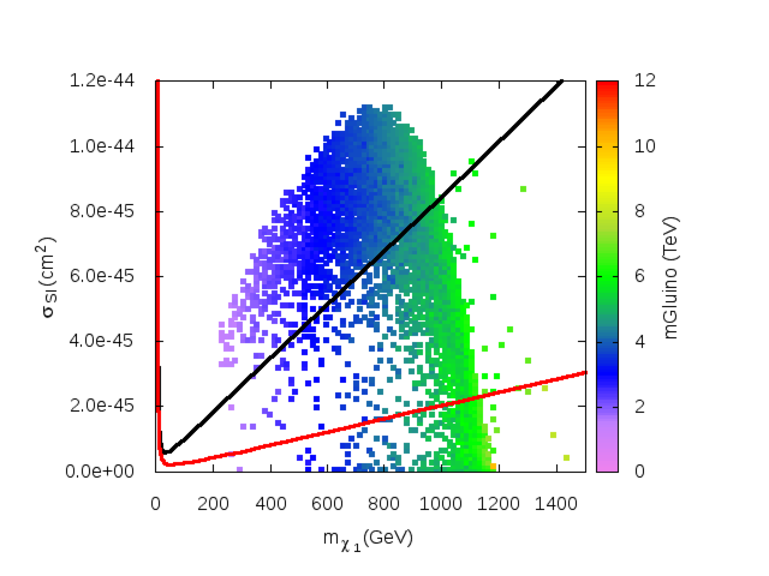
\includegraphics[width=0.45\textwidth]{ezssm_direct_detection}
    \hfill
    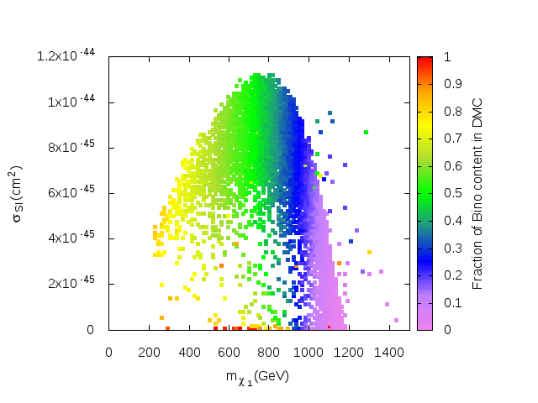
\includegraphics[width=0.45\textwidth]{ezssm_bino_fraction}
    \hfill
  \end{figure}
  \vspace*{-20pt}
  \begin{center}
    { \tiny [\href{http://arxiv.org/abs/1611.05966}{%
          arXiv:1611.05966}] }
  \end{center}
  \begin{itemize} \itemsep1em
  \item \alert{Note: none of these $Z_2$ symmetries commute with $E_6$}
  \end{itemize}
      {\tiny [2] J.~P.~Hall and S.~F.~King,
        \href{http://doi.org/10.1007/JHEP06(2011)006}{JHEP
          \textbf{1106}, 006 (20011)}
        (\href{http://arxiv.org/abs/1104.2259}{arXiv:1104.2259})}
\end{frame}

\section{The SE$_6$SSM}

\begin{frame}
  \frametitle{The SE$_6$SSM}
  \begin{itemize} \itemsep1em
    \item $E_6$ inspired model arising from 5D or 6D orbifold GUT [3]
    \item Complete $\mathbf{27}$-plets supplemented by components
      of {\color{orange} extra $\mathbf{27^\prime}$-,
        $\mathbf{\overline{27}^\prime}$-plets}
    \item Stabilise Higgs potential $\Rightarrow$ pure singlet $\hat{\phi}$

    \item $U(1)_\psi \times U(1)_\chi \rightarrow U(1)_N \times Z_2^M$
      at intermediate scale $\Rightarrow$ {\color{blue} automatically conserved
        $Z_2^M$}
    \item $Z_2^{B/L}$, $Z_2^H$ superseded by
      {\color{blue} single exact $\tilde{Z}_2^H$}
  \end{itemize}
  \vspace*{8pt}
  \begin{empheq}[box=\widefbox]{align*}
    W_{\text{SE}_6\text{SSM}} = {} & \, \lambda {\color{orange} \hat{S}}
    ({\color{orange}\hat{H}_d} \cdot {\color{orange} \hat{H}_u})
    - \sigma \hat{\phi} {\color{orange}\hat{S}}
    {\color{orange}\hat{\overline{S}}}
    + \frac{\kappa}{3}\hat{\phi}^3 + \frac{\mu}{2}\hat{\phi}^2
    + \Lambda_F\hat{\phi} + \lambda_{\alpha\beta} {\color{orange}\hat{S}}
    (\hat{H}^d_{\alpha} \cdot \hat{H}^u_{\beta}) \\
    & {} + \kappa_{ij} {\color{orange}\hat{S}}
    \hat{D}_{i} \hat{\overline{D}}_{j}
    + \tilde{f}_{i\alpha} \hat{S}_{i} ({\color{orange}\hat{H}_u} \cdot
    \hat{H}^d_{\alpha}) + f_{i\alpha} \hat{S}_{i} (\hat{H}^u_{\alpha}
    \cdot {\color{orange}\hat{H}_d})
    + g^D_{ij} (\hat{Q}_i \cdot {\color{orange}\hat{L}_4})
    \hat{\overline{D}}_j \\
    & {} + h^E_{i\alpha} \hat{e}^c_{i} (\hat{H}^d_{\alpha} \cdot
    {\color{orange}\hat{L}_4})
    + \mu_L({\color{orange}\hat{L}_4} \cdot
    {\color{orange}\hat{\overline{L}}_4}) + \tilde{\sigma}
    \hat{\phi} ({\color{orange}\hat{L}_4} \cdot
    {\color{orange}\hat{\overline{L}}_4})
    + W_{\text{MSSM}}(\mu=0)
  \end{empheq}
  \vfill
  {\tiny [3] R.~Nevzorov,
        \href{http://doi.org/10.1103/PhysRevD.87.015029}
             {Phys. Rev. \textbf{D} 87, 015029 (2013)}
             (\href{http://arxiv.org/abs/1205.5967}{arXiv:1205.5967})}
\end{frame}

\begin{frame}
  \frametitle{DM Candidates?}
  \begin{columns}[t]
    \begin{column}{0.6\textwidth}
      \begin{itemize} \itemsep1.2em
      \item Conserved $Z_2^M$, $\tilde{Z}_2^H$ $\Rightarrow$
        \emph{two} (distinct) DM candidates
        \item ``Exotics'' $\equiv Z_2^E$ odd states, where
          $\tilde{Z}_2^H = Z_2^M \times Z_2^E$
      \item $Z_2^E$ conserved $\Rightarrow$ lightest exotic is stable
      \item Limits from exotic Higgs decays, DM direct detection
        $\Rightarrow$ inert singlinos $\tilde{S}_i$ form subdominant hot DM,
        $m_{\tilde{S}_i} \ll 1$ eV
      \item $M_{Z'} \gg M_S \gg M_Z$ $\Rightarrow$ {\color{orange}
        singlet dominated $\tilde{\chi}^0$'s} decouple
      \item $\Rightarrow$ allowed scenarios have
        {\color{blue} MSSM-like $\tilde{\chi}_1^0$} as LSP
        \begin{itemize} \itemsep0.5em
        \item Permits interesting comparison with MSSM
        \item Explore parameter space of constrained models
        \end{itemize}
      \end{itemize}
    \end{column}
    \begin{column}{0.4\textwidth}
      \begin{table}[ht]
        \centering
        \small
        \begin{tabular}{cccc}
          \toprule
          & $\tilde{Z}_2^H$ & $Z_2^M$ & $Z_2^E$ \\
          \midrule
          $\hat{Q}_i$, $\hat{u}_i^c$, $\hat{d}_i^c$, $\hat{L}_i$, $\hat{e}_i^c$,
          $\hat{N}_i^c$ & $-$ & $-$ & $+$ \\
          $\hat{H}_{\alpha}^u$, $\hat{H}_{\alpha}^d$, $\hat{S}_i$,
          $\hat{D}_i$, $\hat{\overline{D}}_i$ & $-$ & $+$ & $-$ \\
          $\hat{H}_u$, $\hat{H}_d$ & $+$ & $+$ & $+$ \\
          $\hat{S}$, $\hat{\overline{S}}$ & $+$ & $+$ & $+$ \\
          $\hat{L}_4$, $\hat{\overline{L}}_4$ & $+$ & $-$ & $-$ \\
          \bottomrule
        \end{tabular}
      \end{table}
      \vspace{4pt}
      \begin{center}
        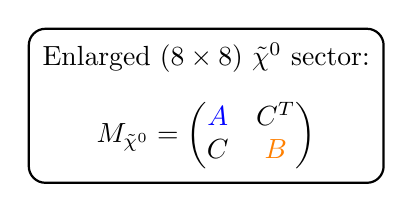
\begin{tikzpicture}
          \node[rectangle, draw, fill = white, rounded corners = 6pt,
            thick, inner sep = 0.5em,align = center]{%
            Enlarged ($8 \times 8$) $\tilde{\chi}^0$ sector:\\[1em]
            $
            M_{\tilde{\chi}^0} = \begin{pmatrix}
              {\color{blue} A} & C^T \\
              C & {\color{orange} B}
            \end{pmatrix}
            $
          };
        \end{tikzpicture}
      \end{center}
    \end{column}
  \end{columns}
\end{frame}

\section{Results}

\begin{frame}
  \frametitle{Parameter Space Restrictions}
  \begin{columns}[t]
    \begin{column}{0.3\textwidth}
      \vspace{-37pt}
      \begin{figure}
        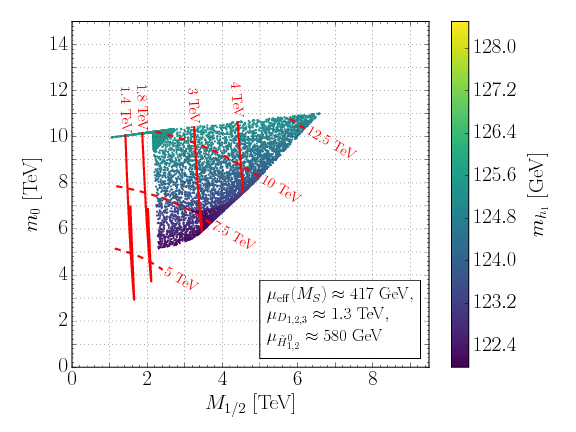
\includegraphics[width=1.1\textwidth]{cse6ssm_mupos400GeV_m12m0_Mhh}
      \end{figure}
      \vspace{-30pt}
      \begin{figure}
        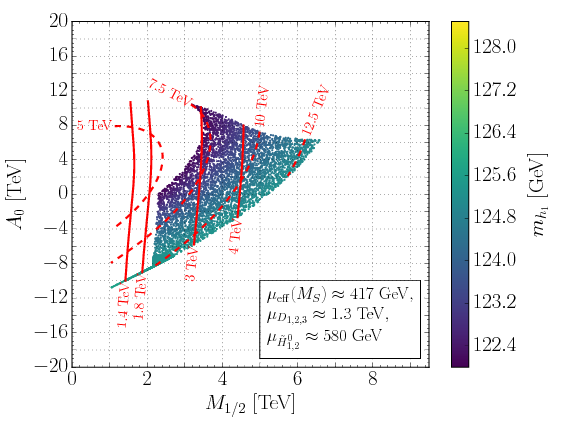
\includegraphics[width=1.1\textwidth]{cse6ssm_mupos400GeV_m12A0_Mhh}
      \end{figure}
      \vspace{-22pt}
      \begin{center}
        \tiny [\href{https://arxiv.org/abs/1610.03374}{arXiv:1610.03374}]
      \end{center}
    \end{column}
    \begin{column}{0.7\textwidth}
      \vspace{-15pt}
      \begin{columns}[t]
        \begin{column}{0.5\textwidth}
          \vspace{-32pt}
          \begin{figure}
            \hspace*{20pt}
            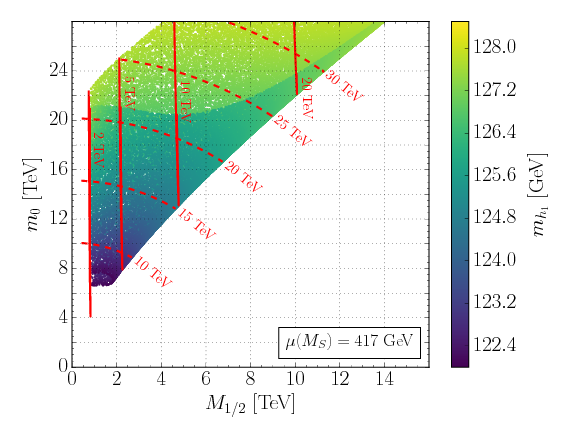
\includegraphics[width=0.93\textwidth]{cmssm_mupos400GeV_m12m0_Mhh}
          \end{figure}
        \end{column}
        \begin{column}{0.5\textwidth}
          \vspace{-20pt}
          \begin{figure}
            \centering
            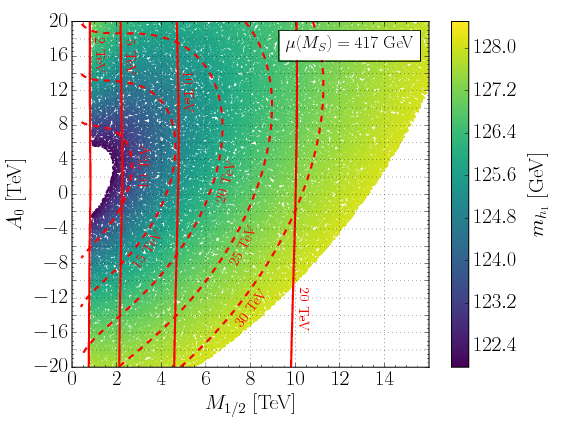
\includegraphics[width=0.92\textwidth]{cmssm_mupos400GeV_m12A0_Mhh}
          \end{figure}
        \end{column}
      \end{columns}
      \begin{itemize}
      \item Successful EWSB $+$ $m_{h_1} \approx 125$ GeV $\Rightarrow$
        large $m_0 > M_{1/2}, A_0$
      \item \alert{$m_{h_1} \approx 125$ GeV important constraint on
        range of variation of $M_{1/2}$, $A_0$}
        \begin{itemize}
        \item Additional constraints in CSE$_6$SSM from tachyonic
          CP-even and CP-odd Higgs states
        \end{itemize}
      \item More generally: {\color{blue} $m_{h_1}$ constraint
        should not be ignored in BSM models}
        \begin{itemize} \itemsep0.5em
        \item Expt. precision $\Rightarrow$ \alert{precise theoretical
          calculation required}
        \item E.g., on-going work on CNMSSM, CE$_6$SSM
        \end{itemize}
      \end{itemize}
    \end{column}
  \end{columns}
\end{frame}

\begin{frame}
  \frametitle{Sparticle Mass Spectrum}
  \begin{columns}[t]
    \begin{column}{0.4\textwidth}
      \vspace{-30pt}
      \begin{figure}
        \begin{center}
          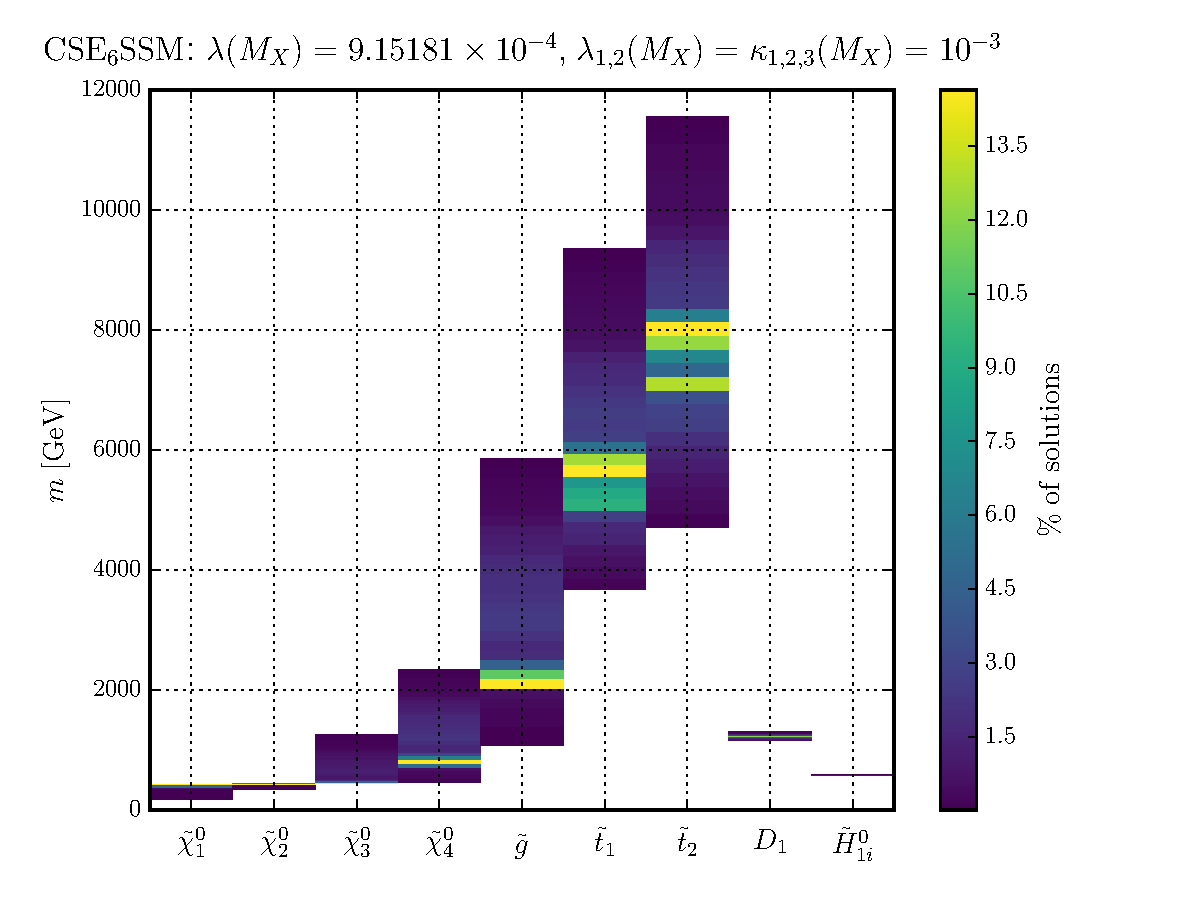
\includegraphics[width=6.5cm]{cse6ssm_300GeV_mueff_spectrum}
        \end{center}
      \end{figure}
    \end{column}
    \begin{column}{0.6\textwidth}
      \vspace{-10pt}
      \begin{itemize} \itemsep1em
      \item Sfermions heavy, but gluino and EW-inos
        can be observable
      \item Extra matter content $\supset$ inert states $+$ exotic leptons
        $\hat{L}_4$, $\hat{\overline{L}}_4$, spin-$0$, spin-$1/2$
        leptoquarks $\hat{D}_i$, $\hat{\overline{D}}_i$
      \item {\color{blue} Light exotic fermions can be observable}
        \begin{itemize} \itemsep0.8em
        \item Exotic leptoquarks $D_i$: e.g., $p\,p \to t\,\bar{t}
          \,\tau^+\,\tau^-+E_T^{miss}+X$,
          $p\,p \to b\,\bar{b} + E_T^{miss} + X$
        \item Charged, neutral inert Higgsinos: e.g., $p\,p\to W\,W / Z\,Z
          / W\,Z +E_T^{miss}+X$
        \end{itemize}
      \end{itemize}
    \end{column}
  \end{columns}
  \vspace{2pt}
  \begin{center}
    \begin{figure}
      \includegraphics[width=0.16\textwidth]{leptoquarkdecay}
      \hspace{40pt}
      \includegraphics[width=0.16\textwidth]{exoticsleptondecay}
      \hspace{40pt}
      \includegraphics[width=0.16\textwidth]{inerthiggsinodecay1}
      \hspace{40pt}
      \includegraphics[width=0.16\textwidth]{inerthiggsinodecay2}
    \end{figure}
  \end{center}
\end{frame}

\begin{frame}
  \frametitle{$\mu_{(\text{eff.})} \approx 400$ GeV: Relic Density}
  \begin{columns}[t]
    \begin{column}{0.5\textwidth}
      \vspace{-16pt}
      \begin{figure}
        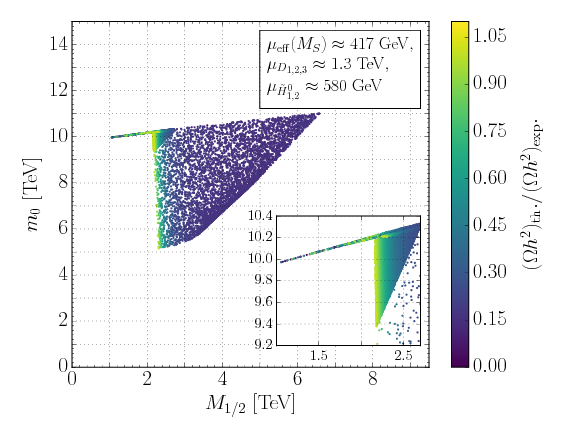
\includegraphics[width=\textwidth]{cse6ssm_mupos400GeV_m12m0_Omega}
      \end{figure}
      \vspace{-12pt}
      \begin{itemize}
        \item $\Omega h^2 \approx 0.1187$ $\Rightarrow$ ``well-tempered''
          bino-Higgsino $\tilde{\chi}^0$ ($\mu_{\text{eff.}} \sim M_1$)
        \item Pair annihilations $\tilde{\chi}_1^0\,\tilde{\chi}_1^0
          \rightarrow \bar{f}\,f$
      \end{itemize}
    \end{column}
    \begin{column}{0.5\textwidth}
      \vspace{-23pt}
      \begin{center}
        \tiny [\href{https://arxiv.org/abs/1610.03374}{arXiv:1610.03374}]
      \end{center}
      \vspace{-19pt}
      \begin{figure}
        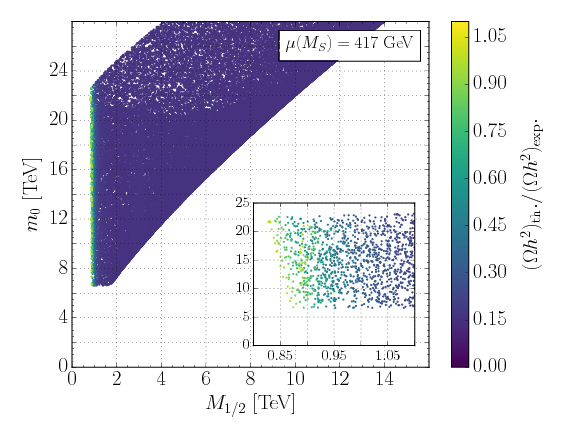
\includegraphics[width=\textwidth]{cmssm_mupos400GeV_m12m0_Omega}
      \end{figure}
      \vspace{-13pt}
      \begin{itemize}
        \item MSSM-like nature of neutralino sector clear $-$
          almost identical behaviour
        \item {\color{blue} Existence of $A$-funnel at $\tan\beta = 10$ notable
          difference in CSE$_6$SSM}
      \end{itemize}
      \end{column}
  \end{columns}
\end{frame}

\begin{frame}
  \frametitle{$\mu_{(\text{eff.})} \approx 400$ GeV: Direct Detection
    Cross Section}
  \begin{columns}[t]
    \begin{column}{0.6\textwidth}
      \vspace{-25pt}
      \begin{figure}
        \includegraphics[width=0.82\textwidth]{%
          cse6ssm_mupos400GeV_m12m0_SigmaSIProton}
      \end{figure}
      \vspace*{-12pt}
      \begin{itemize}
      \item $\sigma^{SI}$ set by $g_{h_1 \chi_1 \chi_1}$ ($t$-channel $h$
        exchange):
        {
          \begin{equation*}\hspace*{-15pt}
            g_{h_1 \chi_1 \chi_1} \approx \frac{1}{2} \left (
            \sqrt{\frac{3}{5}} g_1
                 {\color{red} N_{14}}
                 - g_2 N_{13} \right ) \left [ {\color{red}N_{11}}
                   (U_h)_{11} - {\color{red}N_{12}} (U_h)_{12}
                   \right ]
        \end{equation*}}
      \end{itemize}
    \end{column}
    \begin{column}{0.4\textwidth}
      \vspace{-10pt}
      \begin{itemize}
        \item Well-tempered $\tilde{\chi}^0_1$ $\Rightarrow$ large
          mixing, {\color{red}$\sigma_{SI}$ exceeds, e.g., $90$\% LUX
            limits}
        \item $M_1 \gg \mu_{\text{eff.}}$ both mixing and number density
          suppressed
      \end{itemize}
      \vspace{-8pt}
      \begin{figure}
        \includegraphics[width=1.07\textwidth]{%
          cmssm_mupos400GeV_m12m0_SigmaSIProton}
      \end{figure}
      \vspace{-20pt}
      \begin{center}
        \tiny [\href{https://arxiv.org/abs/1610.03374}{arXiv:1610.03374}]
      \end{center}
    \end{column}
  \end{columns}
\end{frame}

\begin{frame}
  \frametitle{$\mu_{(\text{eff.})} \approx 1$ TeV: Pure Higgsino DM
    Candidate}
    \begin{columns}[t]
    \begin{column}{0.3\textwidth}
      \vspace{-35pt}
      \begin{figure}
        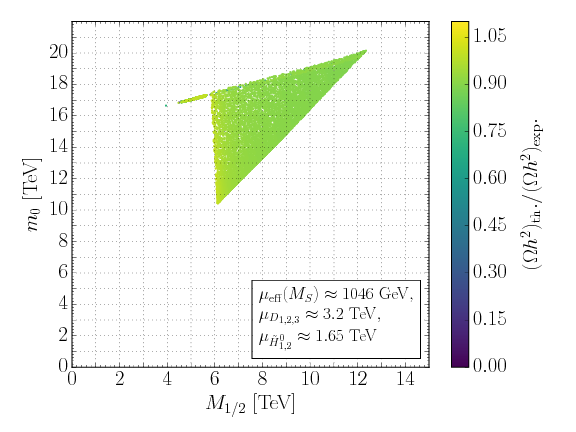
\includegraphics[width=1.1\textwidth]{cse6ssm_mupos1TeV_m12m0_Omega}
      \end{figure}
      \vspace{-30pt}
      \begin{figure}
        \includegraphics[width=1.1\textwidth]{%
          cse6ssm_mupos1TeV_m12m0_SigmaSIProton}
      \end{figure}
      \vspace{-20pt}
      \begin{center}
        \tiny [\href{https://arxiv.org/abs/1610.03374}{arXiv:1610.03374}]
      \end{center}
    \end{column}
    \begin{column}{0.7\textwidth}
      \begin{columns}[t]
        \begin{column}{0.5\textwidth}
          \vspace{-47pt}
          \begin{figure}
            \hspace*{20pt}
            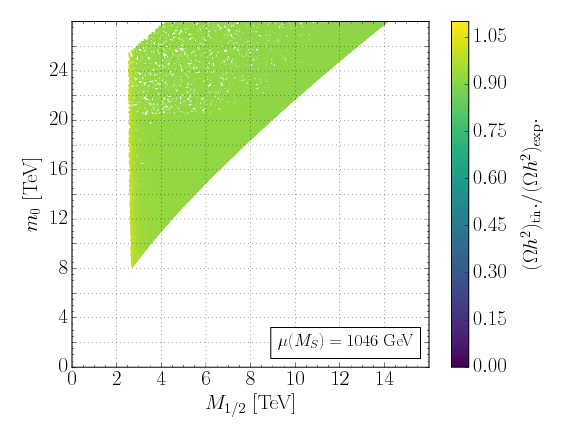
\includegraphics[width=0.93\textwidth]{cmssm_mupos1TeV_m12m0_Omega}
          \end{figure}
        \end{column}
        \begin{column}{0.5\textwidth}
          \vspace{-35pt}
          \begin{figure}
            \centering
            \includegraphics[width=0.92\textwidth]{%
              cmssm_mupos1TeV_m12m0_SigmaSIProton}
          \end{figure}
        \end{column}
      \end{columns}
      \begin{itemize}\itemsep1em
        \item Similar parameter space constraints due to $m_{h_1}$,
          tachyonic states
        \item Suppress $\tilde{B}$ fraction $\Rightarrow$
          large $M_{1/2}$, {\color{red} $m_{\tilde{g}} \gtrsim 4$ TeV,
          $m_{\tilde{q}} \gtrsim 10$ TeV}
        \item {\color{blue} Exotics not forced to be heavy}
        \item $\sigma^{SI}$ (mostly) acceptably small
      \end{itemize}
    \end{column}
  \end{columns}
\end{frame}

\begin{frame}
  \frametitle{Current and Future Limits}
  \begin{columns}[t]
    \begin{column}{0.5\textwidth}
      \vspace{-12pt}
      \begin{figure}
        \includegraphics[width=0.9\textwidth]{%
          cse6ssm_mupos400GeV_MGluMSu6_exclusions}
      \end{figure}
      \vspace*{-8pt}
      \begin{itemize}\itemsep1em
        \item {\color{red} LUX $\Rightarrow$ already stringent limits
          on highly mixed scenarios}
        \item XENON1T expected to cover many of the remaining
          solutions
      \end{itemize}
    \end{column}
    \begin{column}{0.5\textwidth}
      \vspace{-24pt}
      \begin{center}
        \tiny [\href{https://arxiv.org/abs/1610.03374}{arXiv:1610.03374}]
      \end{center}
      \vspace{-12pt}
      \begin{figure}
        \includegraphics[width=0.9\textwidth]{%
          cmssm_mupos400GeV_MGluMSu6_exclusions}
      \end{figure}
      \vspace*{-8pt}
      \begin{itemize}\itemsep1em
        \item SD limits (LUX, IceCube) can also be relevant
        \item $A$-funnel solutions can survive, but in reach of
          LHC run II $\Rightarrow$ {\color{blue}
            complementarity of searches}
      \end{itemize}
    \end{column}
  \end{columns}
\end{frame}

\begin{frame}
  \frametitle{Current and Future Limits}
  \begin{columns}[t]
    \begin{column}{0.5\textwidth}
      \vspace{-22pt}
      \begin{figure}
        \includegraphics[width=0.9\textwidth]{%
          cse6ssm_mupos1TeV_MGluMSu6_exclusions}
      \end{figure}
      \vspace*{-8pt}
      \begin{itemize}\itemsep1em
        \item Essentially no collider limits for $\mu_{\text{eff.}}
          \approx 1$ TeV ({\color{blue}except possibly exotics})
        \item {\color{red} LUX now excludes mixed
          $\tilde{\chi}_1^0$ even when $m_{\tilde{\chi}_1^0} \approx 1$ TeV}
      \end{itemize}
    \end{column}
    \begin{column}{0.5\textwidth}
      \vspace{-22pt}
      \begin{itemize}\itemsep1em
        \item Non-mixed scenarios expected to be discoverable at
          XENON1T
        \item Larger $M_{1/2}$ and heavy exotics $\Rightarrow$ only
          accessible at, e.g., LZ
      \end{itemize}
      \begin{figure}
        \includegraphics[width=0.9\textwidth]{%
          cmssm_mupos1TeV_MGluMSu6_exclusions}
      \end{figure}
      \vspace{-20pt}
      \begin{center}
        \tiny [\href{https://arxiv.org/abs/1610.03374}{arXiv:1610.03374}]
      \end{center}
    \end{column}
  \end{columns}
\end{frame}

\section{Summary}

\begin{frame}
  \frametitle{Summary}
  \begin{itemize} \itemsep1em
  \item $E_6$ inspired models are well-motivated extensions of the MSSM,
    addressing, e.g., little hierarchy problem, $\mu$-problem, $\ldots$
  \item Novel DM scenarios involving inert states viable in simplest $E_6$
    models, but require multiple discrete symmetries
  \item SE$_6$SSM is a well-motivated extension with an exact custodial
    symmetry
  \item DM relic density can be fitted by MSSM-like $\tilde{\chi}_1^0$, with
    e.g., $\tilde{\chi}_1^0$ bino-Higgsino or pure Higgsino
  \item Direct detection searches $\Rightarrow$ \alert{stringent limits on
    allowed mixing}
  \item XENON1T expected to probe much of remainder space, {\color{blue}
    complementary probe to LHC searches}
  \item {\color{blue} $E_6$ exotics not required to be heavy
    $\Rightarrow$ possible means of constraining/discovering model}
  \end{itemize}
  \begin{center}
    \large Thank you for listening!
  \end{center}
\end{frame}

\appendix

\begin{frame}
  \begin{center}
    {
      \Large
      Additional Slides
    }
  \end{center}
\end{frame}

\begin{frame}
  \frametitle{The CSE$_6$SSM}
  \begin{itemize}
    \vfill
    \item {\color{red} General model is complicated}
          \begin{itemize}
            \item $O(200)$ new parameters (assuming no new sources of
                  CP-violation)
            \item Many masses and mixings
          \end{itemize}
    \vfill
    \item Consider constrained model (CSE$_6$SSM) inspired by gravity
          mediated SUSY breaking
    \vfill
  \item {\color{blue} Universal soft breaking parameters: $M_{1/2}$, $A_0$,
    $B_0$, $m_0$}
    \vfill
    \item Interested in mechanism decoupling $Z^\prime$ from EWSB conditions
          $\Rightarrow$ can have large $s = \sqrt{s_1^2 + s_2^2}$
    \vfill
    \item Higgsino mass set by $\mu_{\text{eff}} = \lambda s_1 / \sqrt{2}$
      $\Rightarrow$ acceptable LSP mass ($\lesssim$ TeV) for small
      $\lambda$
    \vfill
    \item $\Rightarrow$ other exotic couplings must be small,
          otherwise exotic states are tachyonic
  \end{itemize}
\end{frame}

\begin{frame}
  \frametitle{Parameter Space Scans}
  \begin{itemize}\itemsep1em
    \item Focus on heavy $Z^\prime$, $s = 650$ TeV, choose fixed
      $\mu_{\text{eff}}$
    \item Achieve using semi-analytic solutions for soft parameters:
      \begin{align*}
        M_i(Q) &= p_i(Q) M_{1/2} + q_i(Q) A_0 \, , \quad
        A_i(Q) = e_i(Q) A_0 + f_i(Q) M_{1/2} \, , \\
        m_i^2(Q) &= a_i(Q) m_0^2 + b_i(Q) M_{1/2}^2 + c_i(Q) A_0 M_{1/2}
        + d_i(Q) A_0^2 \, , \, \ldots
      \end{align*}
    \item Fix $m_0$ from EWSB,
      $m_0^2 \sim -\frac{b_{H_u}}{a_{H_u}} M_{1/2}^2 - \ldots$
    \item Implemented in FlexibleSUSY for {\color{blue} full 1-loop masses
      and 2-loop RGEs}
      \begin{itemize}
      \item Resulting ``semi-analytic solver'' forms part of
        FlexibleSUSY 2.0 [4], along with many other updates.
      \end{itemize}
    \item Require $\Omega h^2 \leq 0.1187$ (micrOMEGAs) and
      $m_{h_1} = 125.09 \pm 3$ GeV
    \item Compare with CMSSM for $|\mu| \sim 400$ GeV and $|\mu| \sim
      1$ TeV
  \end{itemize}
  \vfill
      {\tiny [4] P.~Athron, M.~Bach, D.~Harries, T.~Kwasnitza,
        J.-h.~Park, D.~St\"{o}ckinger, A.~Voigt, and J.~Ziebell,
        \href{http://arxiv.org/abs/1710.03760}{arXiv:1710.03760}
      }
\end{frame}

\begin{frame}
  \frametitle{$A$-funnel in the CSE$_6$SSM}
  \begin{columns}[t]
    \begin{column}{0.5\textwidth}
      \begin{itemize} \itemsep1.5em
        \vfill
      \item Solutions at lower $M_{1/2}$ due to
        $m_{A_1} \sim 2 m_{\tilde{\chi}_1^0}$
        \vfill
      \item CMSSM: $A$-funnel requires $\tan\beta \gtrsim 40$
        \vfill
      \item CSE$_6$SSM: tune $A_0$ for given $\tan\beta$, $M_{1/2}$ to that
        $m_{A_1} \rightarrow 0$, keeping $m_{\tilde{\chi}_1^0} \sim$ fixed
        \vfill
      \item Lightest state $A_1$ mixture of singlets for $s \gg M_S \gg v$
        ($\tan\delta \approx \frac{s_1 s_2}{\varphi \sqrt{s_1^2 + s_2^2}}$):
        \vfill
      \end{itemize}
    \end{column}
    \begin{column}{0.5\textwidth}
      \vspace{-40pt}
      \begin{figure}
        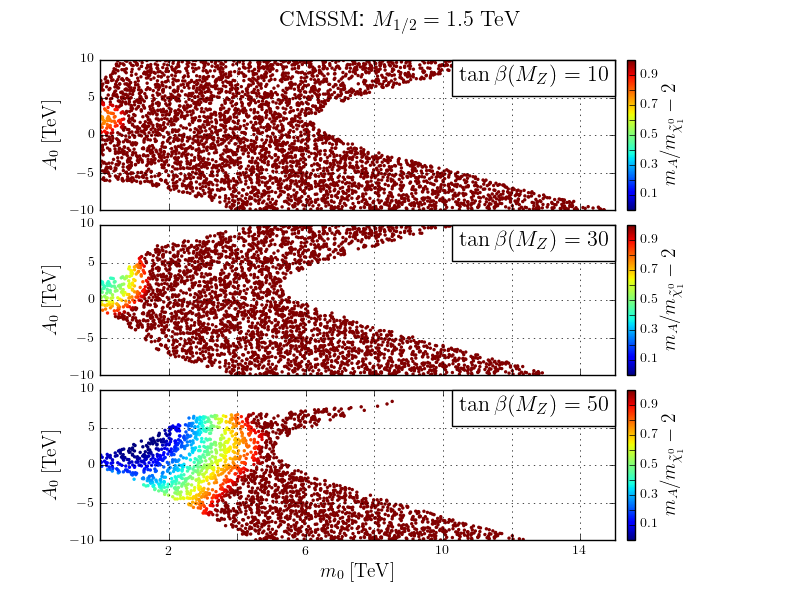
\includegraphics[width=8cm]{cmssm_a_funnel}
      \end{figure}
    \end{column}
  \end{columns}
  \vspace{10pt}
  \begin{equation*}
    m_{A_1}^2 \approx \cos^2\delta \left ( -2 B\mu
    - 3 \frac{\kappa A_\kappa}{\sqrt{2}} \varphi
    - \sqrt{2} \xi \frac{\Lambda}{\varphi} + \frac{9}{2}
    \sigma \kappa s_1 s_2 + 2\sqrt{2} \frac{\sigma \mu s_1 s_2}{\varphi}
    + \frac{\sigma s_1 s_2 \Lambda}{\varphi^2} \right )
  \end{equation*}
\end{frame}

\end{document}
